\documentclass{beamer}
\usefonttheme[onlymath]{serif}
\usepackage{tikz}
\usepackage{graphicx}
\usetheme{metropolis}
\usepackage{lmodern}
\usepackage{amsmath}
\usepackage{mathrsfs}
\usepackage{pdfpages}
\usepackage[backend=biber, style=science]{biblatex}
\addbibresource{/Users/fergusbarratt/bibTex/library.bib}
\graphicspath{ {../../../Images/Presentation/} }

\title{The Dissipative-Driven Jaynes-Cummings System}
\date{\today}
\author{Fergus Barratt}

\begin{document}
\setbeamercolor{block title}{bg=}
\setbeamercolor{block body}{bg=}
\setbeamercolor{background canvas}{bg=}
\maketitle

\begin{frame}

    \frametitle{Superconducting QED}         

    \begin{itemize}
        \item Superconducting CQED is a promising paradigm for the implementation of quantum computers. 
        \item One critical component is the qubit implementation.
        \item In sCQED the canonical example is the Josephson junction qubit, which comes in three kinds, charge, flux, and phase.\footfullcite{Makhlin2001} 
        \item Decoherence is a key problem.
        \item One suggestion is the \emph{transmon}\footfullcite{Blais2004a} a compound system of Josephson qubits.
    \end{itemize}

\end{frame}

\begin{frame}

    \frametitle{The Transmon}

    \includegraphics[scale=0.18, angle=-90, origin=c]{transmon.pdf}
    \includegraphics[scale=0.20, angle=-90, origin=c]{anharmonicity.pdf}

    \begin{itemize}
        \item Figure of merit for qubit candidates is the level anharmonicity 
        \item Increasing anharmonicity generally increases noise.
        \item The transmon can be operated in a regime where noise can be suppressed with only small decreases in anharmonicity  
    \end{itemize}

\end{frame}
\begin{frame}

    \frametitle{Two-Level approximation}

    \begin{itemize}
        \item If we tune the parameters in the problem we can have negligible population of higher levels and an effective qubit.
        \item We put the transmon in a cavity and couple it to light.
        \item This situation is well-described by the Jaynes-Cummings model.
    \end{itemize}

\end{frame}
\begin{frame}

    \frametitle{The Jaynes-Cummings Model}

    \begin{center}
        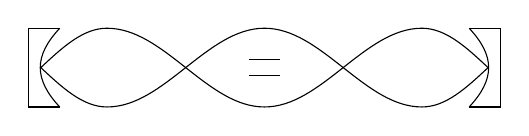
\begin{tikzpicture}[xscale=2]
                \draw (0, 1) -- (0, 0);
                \draw (0, 1) -- (0.2, 1);
                \draw (0, 0) -- (0.2, 0);
                \draw (0.2, 0) to [out=-245, in=245] (0.2, 1);

                \draw (3, 1) -- (3, 0);
                \draw (2.8, 1) -- (3, 1);
                \draw (2.8, 0) -- (3, 0);
                \draw (2.8, 0) to [out=-295, in=295] (2.8, 1);

                \draw (0.08, 0.5) sin (0.5, 1) cos (1, 0.5) sin (1.5, 0) cos (2, 0.5) sin (2.5, 1) cos (2.92, 0.5);

                \draw (0.08, 0.5) sin (0.5, 0) cos (1, 0.5) sin (1.5, 1) cos (2, 0.5) sin (2.5, 0) cos (2.92, 0.5);

                \draw (1.4, 0.4) -- (1.6, 0.4);
                \draw (1.4, 0.6) -- (1.6, 0.6);
        \end{tikzpicture}
    \end{center}

    Single cavity mode interacting with two level system in the RWA. Add coherent drive, dissipation via cavity loss $\kappa$ \& spontaneous emission rate $\gamma$

    \begin{block}{Interaction Hamiltonian}
        $\mathscr{H} = \hbar \delta_{cd} a^\dagger a + \hbar \delta_{qd}\sigma_+ \sigma_- + \hbar g ( a \sigma_+ + a^\dagger \sigma_- ) + \hbar \xi (a + a^\dagger) $
    \end{block}

    \begin{block}{Master Equation}
        $\dot{\rho_S} = \frac{i}{\hbar} [ \mathscr{H}, \rho_S] + \mathscr{L}_{\gamma} [\rho_S] + \mathscr{L}_{\kappa}[\rho_S]$
    \end{block}

\end{frame}
\begin{frame}

    \begin{block}{Resonant}
        $\delta_{cq} = \delta_{cd}=0$
            \footfullcite{Alsing1990}
            \footfullcite{Carmichael2015}
    \end{block}

\end{frame}

\includepdf{resonant.pdf}

\begin{frame}

    \begin{block}{Dispersive}
        $\gamma \ll \kappa \ll g \ll \delta_{cq} \ll \omega_c$
    \end{block}

\end{frame}
\begin{frame}

    \frametitle{The Duffing Oscillator}

    \includegraphics[scale=0.4]{leaf.png}
    \includegraphics[scale=0.4]{scurve.png}

    \begin{itemize}
        \item Transforming the Jaynes Cummings Hamiltonian, dropping terms suppressed with $\frac{1}{\delta_{cq}}$, and ``freezing'' the qubit leaves an approximation to the quantum Duffing Oscillator.
        \item Unlike the Duffing nonlinearity \footfullcite{Drummond1979}, the JC nonlinearity closes with increasing drive\footfullcite{Bishop2010}.
    \end{itemize}

\end{frame}

\includepdf{dispersive.pdf}

\printbibliography\

\end{document}
